\chapter{Imbalanced Classification}
\label{chapter:imb-classif}


\section{Oversampling Methods}
\label{section:oversampling-methods}

Oversampling methods constitute one possible approach to solving the imbalanced classification
problem. The main goal of oversampling methods is to modify the empirical distribution by
increasing the number of samples belonging to the minority class. The empirical distribution is
modified either by duplicating the existing samples or generating new artificial samples until the
desired imbalance ratio is reached. The following text presents oversampling methods used in the
further chapters.


\subsection{Random Oversampling}
\label{subsection:random-oversampling}

The most straightforward approach to tackling the underrepresentation of a class is by duplicating
the available data samples belonging to that class. Samples to duplicate are chosen randomly with a
replacement. Bare duplication of samples may introduce completely overlapping samples, as shown in
the left scatter plot in Figure~\ref{figure:random-oversampling}. Random oversampling introduced
sixty new minority samples to balance the classes; however, we can only see twenty, as most of them
are entirely overlapping. A modification known as \textit{Random Oversampling Examples} (ROSE) was
proposed in 2012 to avoid this~\cite{rose}. It starts by randomly choosing a sample from the
minority class and then generates a new artificial sample in the close neighbourhood of the
original sample. Generating new samples close to the already existing ones enlarges the regions
occupied by the minority class~\cite{smote} and results in a better overall performance of a
classifier.

\begin{figure}
    \centering
    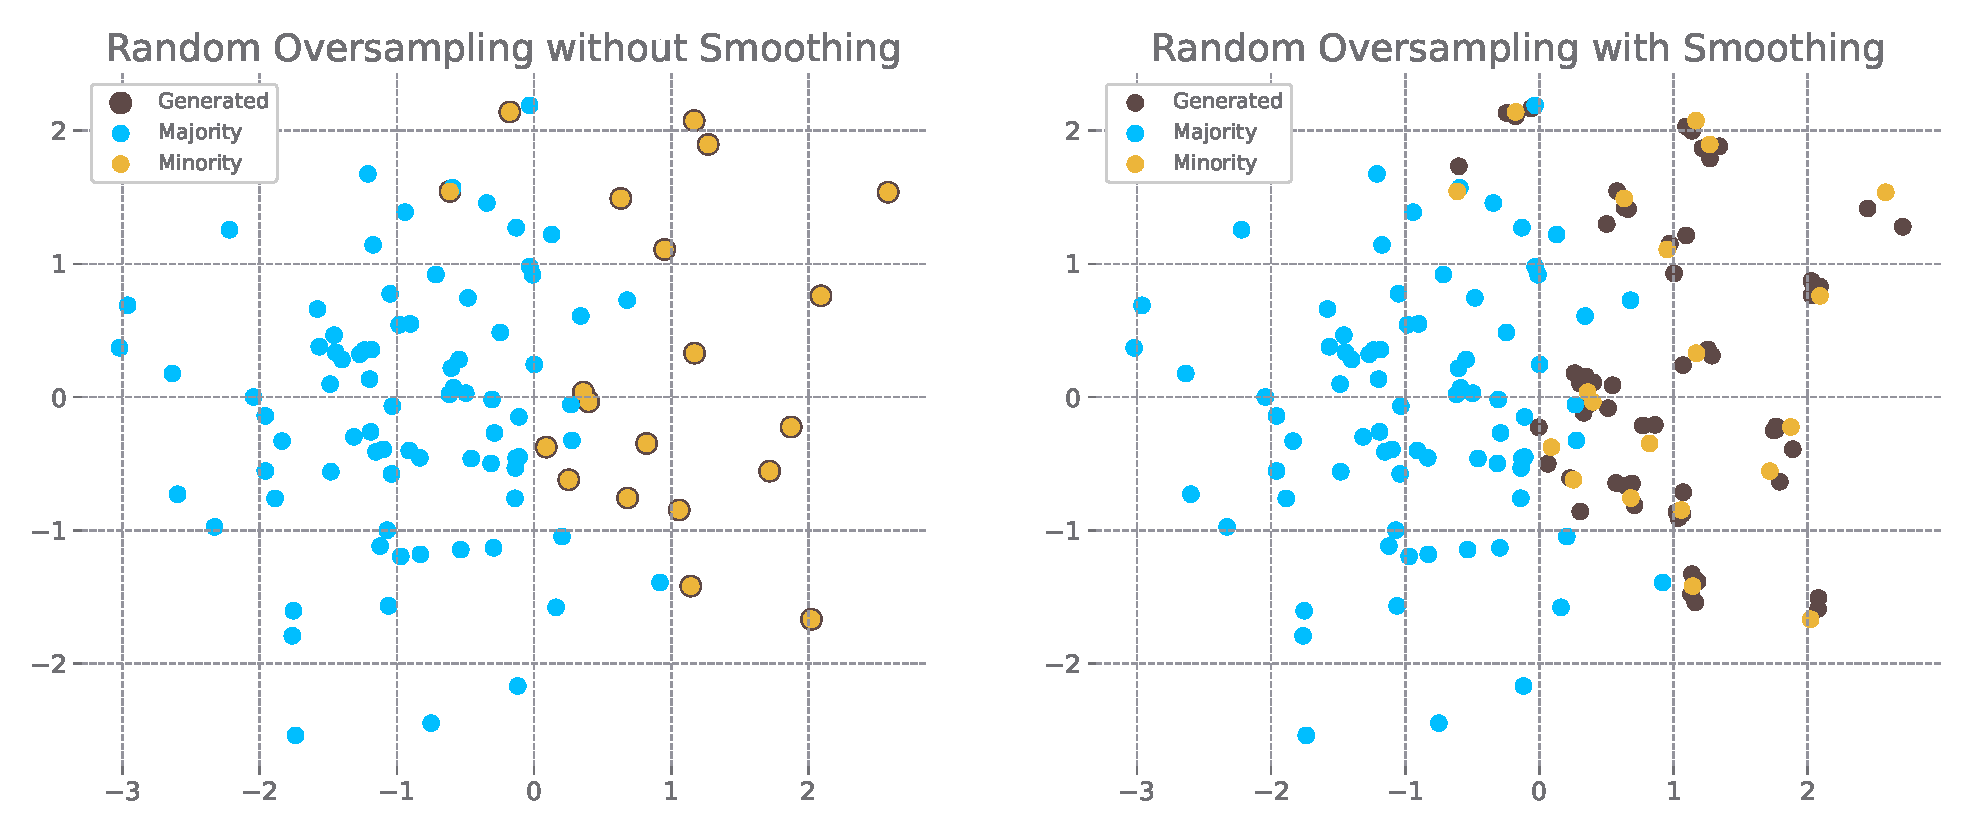
\includegraphics[width=\linewidth]{figures/random_oversampling_vs_rose.eps}
    \caption{
        \textbf{Random Oversampling vs ROSE.} The figure shows how generating new samples in the
        close neighbourhood of the original sample helps to disperse the new samples instead of
        stacking them on top of each other. In both cases, the oversampling method created sixty
        new data samples shown in a brown colour.
    }
    \label{figure:random-oversampling}
\end{figure}


\subsection{Synthetic Minority Oversampling Technique - SMOTE}
\label{subsection:smote}

SMOTE was proposed by Chawla et al.~\cite{smote} in 2002 and is one of the most widely used
imbalanced preprocessing techniques. It creates new synthetic examples on the line segments between
existing examples from the minority class. The amount of oversampling supplied by the user
determines if all minority samples participate in the oversampling. If we plan to oversample the
minority class by at least 100\%, then every existing minority sample is used; otherwise, a random
subset $\mathcal{S} \subseteq {S_{min}}$ of samples is chosen. The algorithm looks at k-nearest
neighbours, where $k$ is again a hyperparameter supplied by the user, of an existing minority
example $\mathbf{x}_i$ and randomly chooses a subset of the neighbours $\mathcal{N} =
\{\,\mathbf{x} \mid \mathbf{x} \in \mathrm{kNN}(\mathbf{x}_i)\,\}$. The subset's size also depends
on the amount of oversampling we plan to do. If, for example, we plan to oversample the minority
class by 200\%, then for each existing minority sample, the subset will contain two randomly chosen
neighbours. If, on the other hand, the amount of oversampling is less than 100\%, the algorithm
generates one new artificial sample for each existing sample in the subset $\mathcal{S}$. For each
neighbour $\mathbf{x}_j \in \mathcal{N}$, the algorithm computes the difference between
$\mathbf{x}_i$ and $\mathbf{x}_j$, multiplies it by a random number $r$ chosen uniformly from the
interval $(0, 1)$, and finally adds it to the original sample $\mathbf{x}_i$. The final formula for
generating a new artificial sample is:
\begin{equation}
    \mathbf{x}_{new} = \mathbf{x}_i + r \cdot (\mathbf{x}_i - \mathbf{x}_j)
    \label{equation:smote}
\end{equation}


\subsection{Borderline SMOTE}
\label{subsection:bordeline-smote}

One drawback the SMOTE algorithm has is that it considers all minority samples to be of the same
importance. Minority samples surrounded largely by majority samples are far more prone to
misclassification than those surrounded predominantly by minority samples. Borderline
SMOTE~\cite{borderline-smote} tries to select only endangered minority samples and performs the
original SMOTE algorithm only on those samples, as shown in
Figure~\ref{figure:smote-vs-borderline}. The algorithm first finds k-nearest neighbours for each
$\mathbf{x}_i \in S_{min}$. Next, it selects only those minority samples with at least half of
their neighbours belonging to the majority class. One interesting case is when all of the
neighbours of a minority sample belong to the majority class. In this case, the minority sample is
considered noise in the data and is not selected. These conditions can be summarised as follow:
\begin{equation}
    \mathcal{S} = \{\mathbf{x} \mid \mathbf{x} \in S_{min} \land \frac{k}{2} \leq \, \mid
        \mathrm{kNN}(\mathbf{x}_i) \cap S_{maj} \mid \, < k\}.
\end{equation}
The resulting set $\mathcal{S}$ is sent to the SMOTE algorithm to generate new artificial samples
on the border.

\begin{figure}
    \centering
    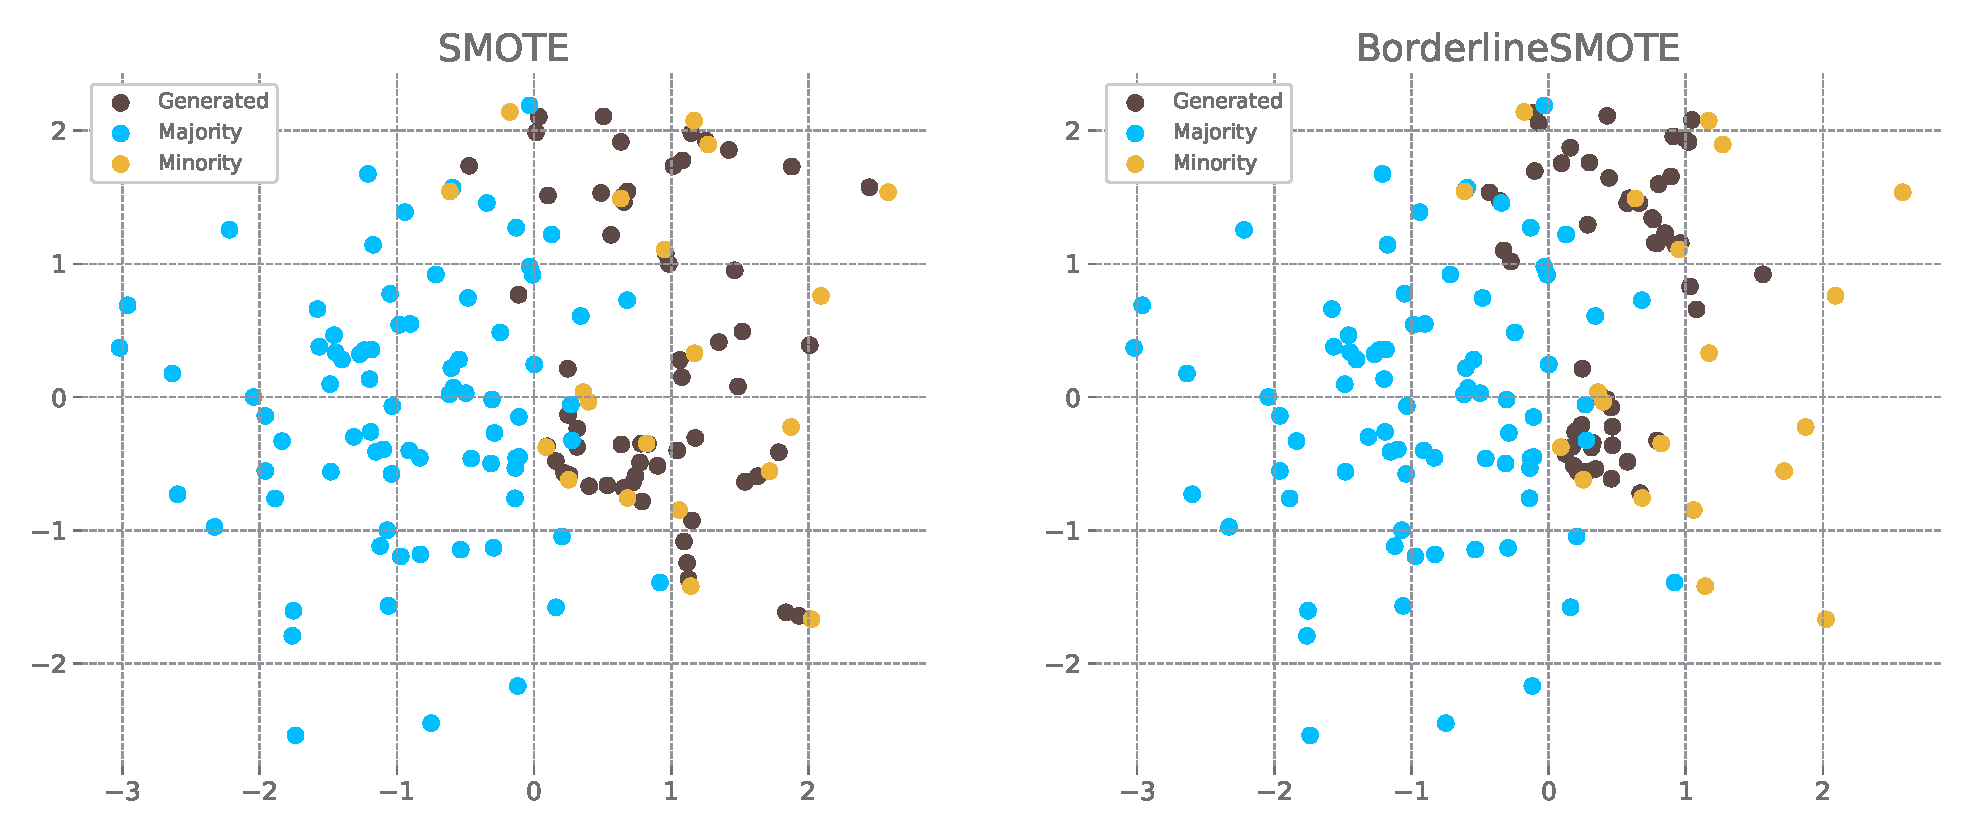
\includegraphics[width=\linewidth]{figures/smote_vs_borderlinesmote.eps}
    \caption{
        \textbf{SMOTE vs Borderline SMOTE.} The figure shows how the Borderline SMOTE algorithm,
        depicted on the right, focuses its attention on endangered minority samples near the
        decision boundary, while SMOTE sees every minority sample having the same importance. The
        most noticeable difference can be seen on the far right side of the figures. SMOTE
        generates new samples in those regions, whereas Borderline SMOTE does not, as those samples
        are far from the decision boundary.
    }
    \label{figure:smote-vs-borderline}
\end{figure}


\subsection{SVM SMOTE}
\label{subsection:svm-smote}

SVM~SMOTE~\cite{svm-smote} also enhances the SMOTE algorithm by focusing on endangered minority
samples. It starts by training a support vector machine classifier~\ref{section:svm} using the
original dataset. The SVM classifier identifies the so-called support vectors in the original data.
These are the training samples that approximate the optimal decision boundary. SVM SMOTE uses these
samples to generate artificial samples near the approximated optimal decision boundary using
interpolation (SMOTE) or extrapolation depending on the density of the majority class around it.
The number of artificial samples to generate is distributed evenly among minority class support
vectors. For each minority support vector $\mathbf{x}_i$, find k-nearest neighbours on the whole
training data set. If minority samples account for less than half of the neighbours, create a new
artificial sample by interpolating between $\mathbf{x}_i$ and its neighbour $\mathbf{x}_j \in
\mathrm{kNN}(\mathbf{x}_i)$ to strengthen the presence of the minority class in crowded regions.
If, on the other hand, there are more minority samples among the neighbours than majority samples,
the algorithm performs extrapolation to enlarge the area occupied by the minority class.

\begin{figure}
    \centering
    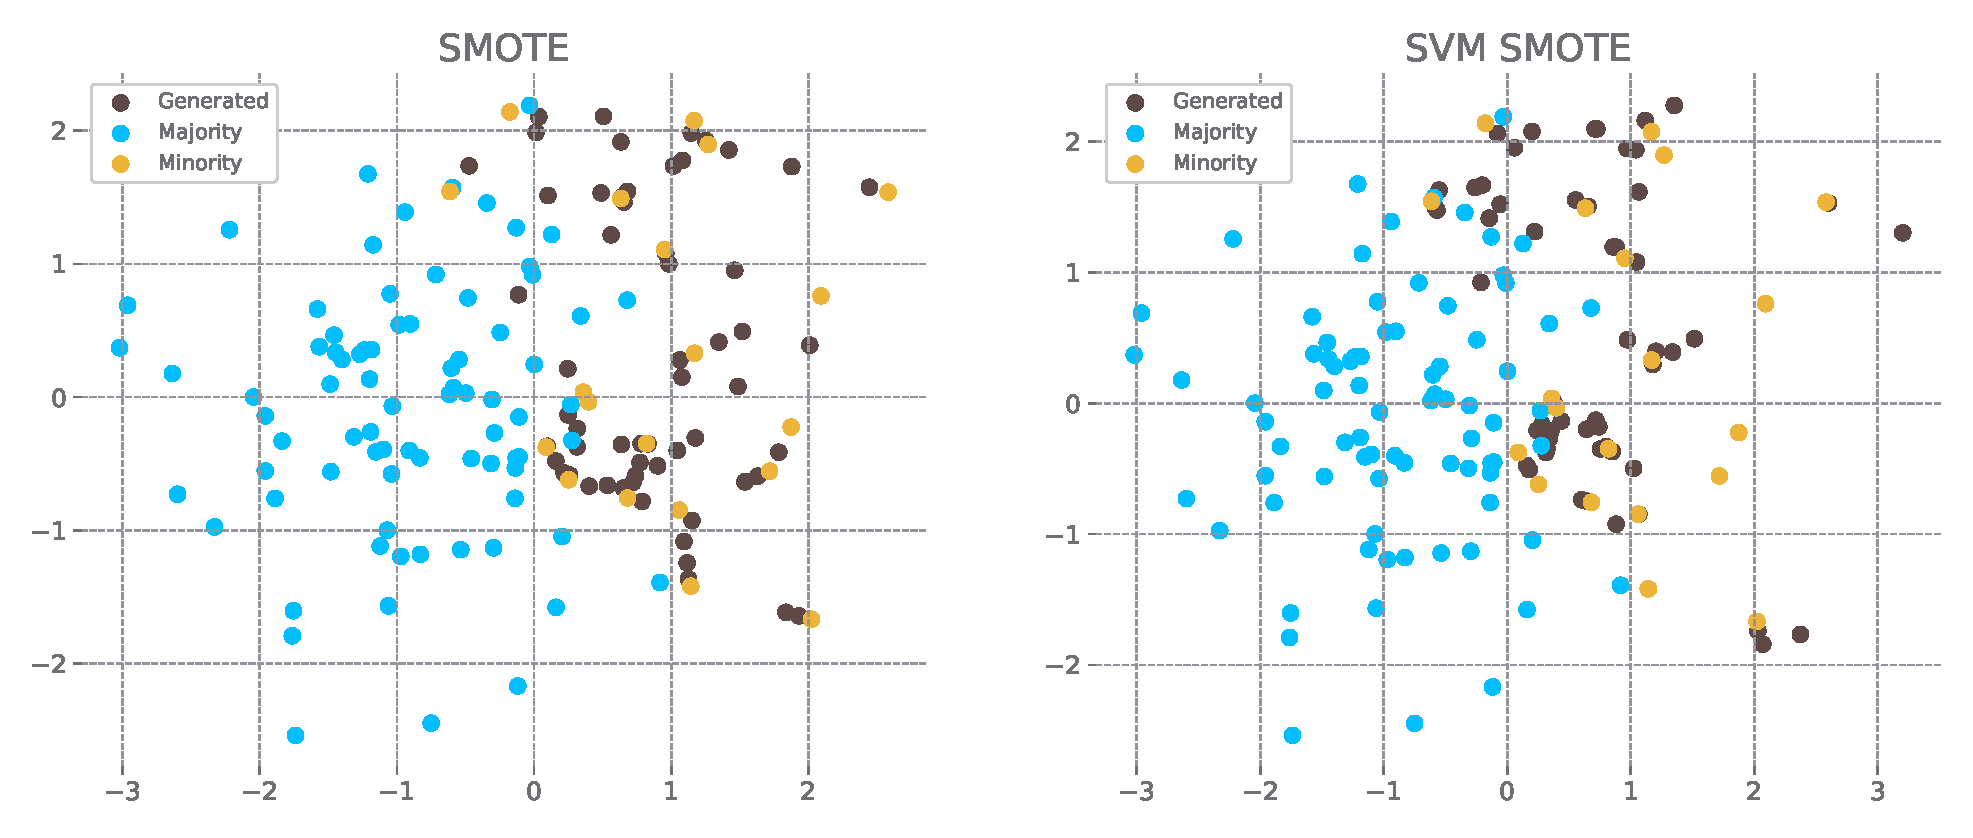
\includegraphics[width=\linewidth]{figures/smote_vs_svmsmote.eps}
    \caption{
        \textbf{SMOTE vs SVM SMOTE.} The figure shows how SVM SMOTE, shown on the right, prefers
        generating samples, shown in a brownish colour, near the decision boundary to strengthen
        the presence of samples from the minority class. In contrast, the original implementation
        of the SMOTE algorithm generates new samples near every original sample from the minority
        class regardless of its position. Furthermore, we can see the interpolation in the dense
        regions in the centre of the plot around the point $(0, 0)$ and the extrapolation on the
        far right.
    }
    \label{figure:smote-vs-svmsmote}
\end{figure}


\subsection{KMeans SMOTE}
\label{subsection:kmeans-smote}

Employing a uniform probability to choose minority samples to oversample is another drawback of
SMOTE. It increases the likelihood of further inflating regions with many minority samples and
neglecting sparse regions~\cite{kmeans-smote}. KMeans~SMOTE~\cite{kmeans-smote} is an enhancement
of SMOTE that focuses on this issue. In the first phase, it employs the KMeans clustering
algorithm~\ref{section:kmeans} to cluster data samples into $k$ groups based on the euclidean
distance. Clustering helps focus the attention on the regions where minority samples are dominant,
preventing SMOTE from generating unnecessary noise by interpolating noisy minority
samples~\cite{kmeans-smote}. Once the clusters were identified, KMeans SMOTE retains only those
clusters that contain more minority samples than majority samples, i.e. clusters whose imbalance
ratio is greater than 1. Next, it computes how many artificial examples must be generated in each
selected cluster based on its density of minority samples. This enables the subsequent step to
generate more samples in sparse regions, thus achieving balanced between-class and
\emph{within-class} distribution. The balanced within-class distribution ensures approximately the
same density of minority samples in the minority class regions. The cluster's density is computed,
for each cluster $f$, as follows:

\begin{enumerate}
    \item calculate a distance matrix between minority samples belonging to cluster $f$
    \item calculate a mean distance $\mathrm{mean\_distance(f)}$
    \item calculate the cluster's density as $\mathrm{density(f)} = \frac{\mid S_{min}
        \mid}{\mathrm{mean\_distance(f)}^m}$, where $m$ is the dimension of a sample
    \item calculate $\mathrm{sparsity(f)} = \frac{1}{\mathrm{density(f)}}$
\end{enumerate}

Finally, normalise $\mathrm{sparsity(f)}$ to be a distribution. Normalisation allows us to multiply
each cluster's sparsity by the total number of data to generate to obtain the portion of samples to
generate in each cluster. The last step of the algorithm consists of performing the SMOTE algorithm
in each cluster separately to generate the needed number of samples to reach the specified ratio of
majority and minority samples.

\begin{figure}
    \centering
    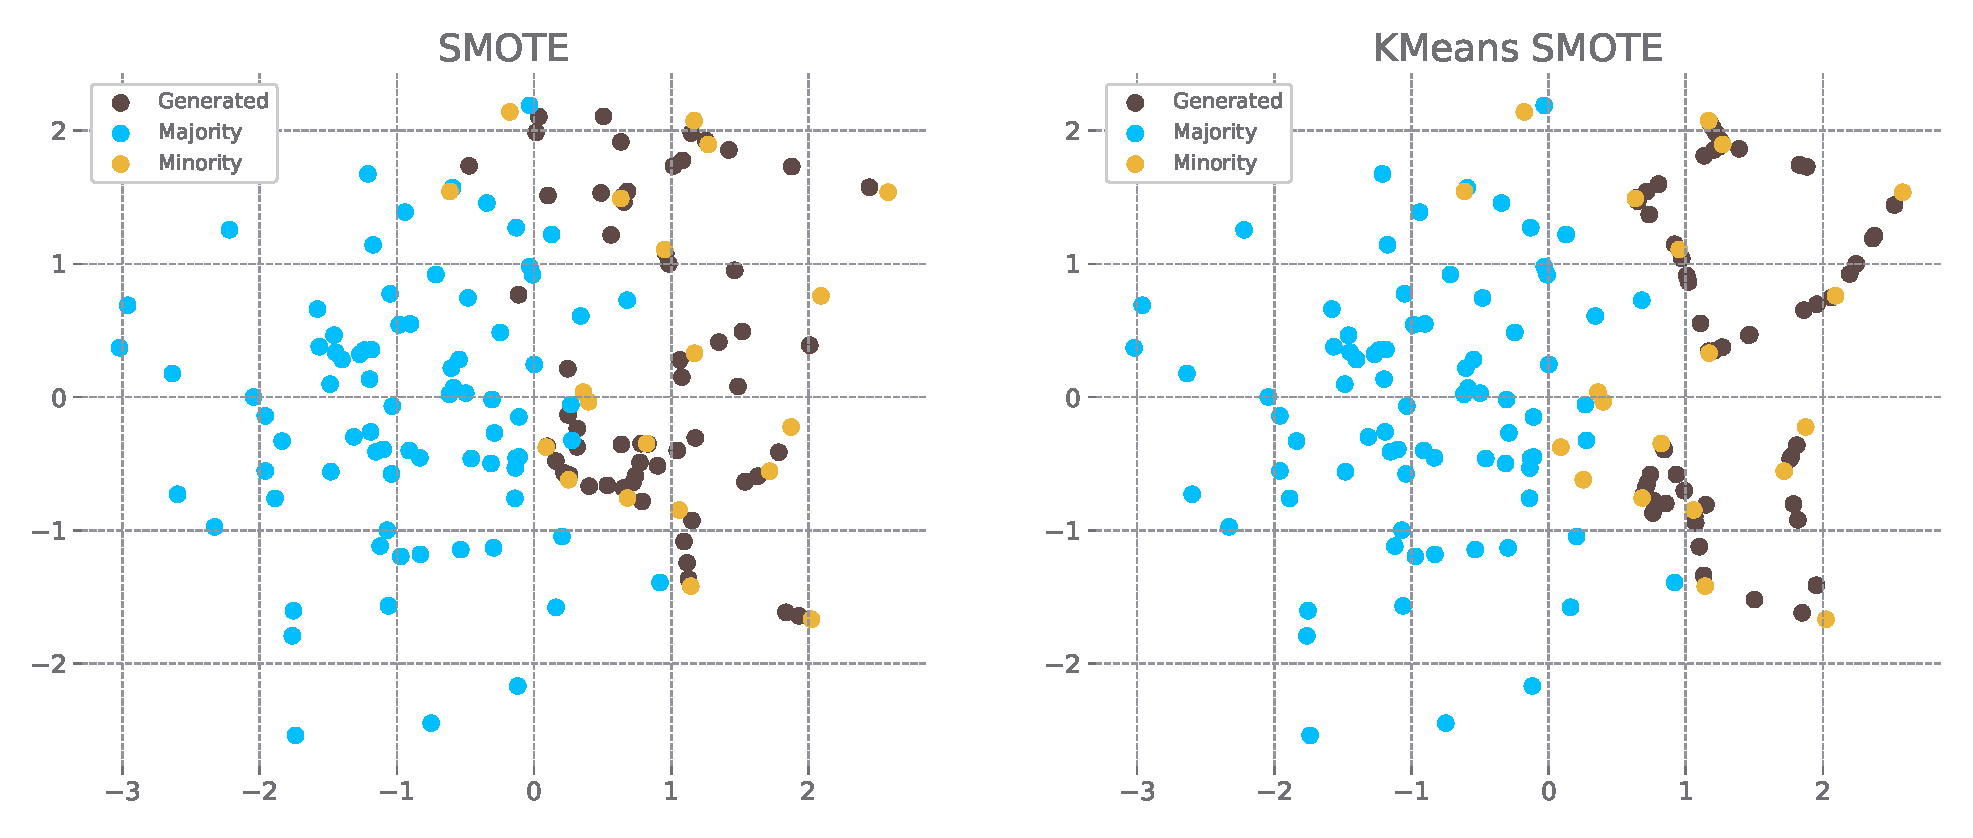
\includegraphics[width=\linewidth]{figures/smote_vs_kmeanssmote.eps}
    \caption{
        \textbf{SMOTE vs KMeans SMOTE.} The figure compares SMOTE and KMeans SMOTE. We can see how
        SMOTE generates many new samples, shown in brown, slightly below the point $(0, 0)$. KMeans
        SMOTE, on the other hand, does not generate almost any new samples in that region as
        samples in that region can be considered noise. The same reasoning can be applied to
        samples at the top, surrounded predominantly by the majority class samples.
    }
    \label{figure:smote-vs-kmeanssmote}
\end{figure}


\subsection{ADASYN}
\label{subsection:adasyn}

Adasyn~\cite{adasyn} assigns a weight to each minority sample based on its difficulty in learning.
Difficulty in learning, in this case, means the portion of k-nearest neighbours that belong to the
opposite class. The greater the number of neighbours of the opposite class, the harder it is to
classify a given minority sample correctly. More synthetic data is generated in areas where it is
hard to learn minority samples, and less data is generated in other, easier-to-learn regions. The
weighting of the minority samples is the main difference between SMOTE and ADASYN, as SMOTE does
not consider the surroundings of minority samples. The ADASYN algorithm starts by calculating the
number of samples that need to be generated using
\begin{equation}
    G = \beta \cdot (\mid S_{maj} \mid - \mid S_{min} \mid),
\end{equation}
where $\beta \in (0, 1)$ controls the level of desired imbalance after resampling.

Next, for each $\mathbf{x}_i \in S_{min}$, find its k-nearest neighbours using the euclidean
distance in the feature space and calculate the portion $r_i$ of the majority samples in the
neighbourhood.
\begin{equation}
    r_i = \frac{\mid \mathrm{kNN}(\mathbf{x}_i) \cap S_{maj} \mid}{k}.
\end{equation}

Normalise $r_i$ to create a proper distribution, i.e. $\sum_{i = 1}^{\mid S_{min} \mid} r_i = 1$.
Normalisation allows us to compute what fraction of all samples that need to be generated should be
generated using each of the minority samples. The number of samples $g_i$ to generate for each
$x_i$ is computed as
\begin{equation}
    g_i = r_i \cdot G.
\end{equation}

Finally, the algorithm uses Equation~\ref{equation:smote} to generate $g_i$ artificial samples for
each minority sample $x_i$.

\begin{figure}
    \centering
    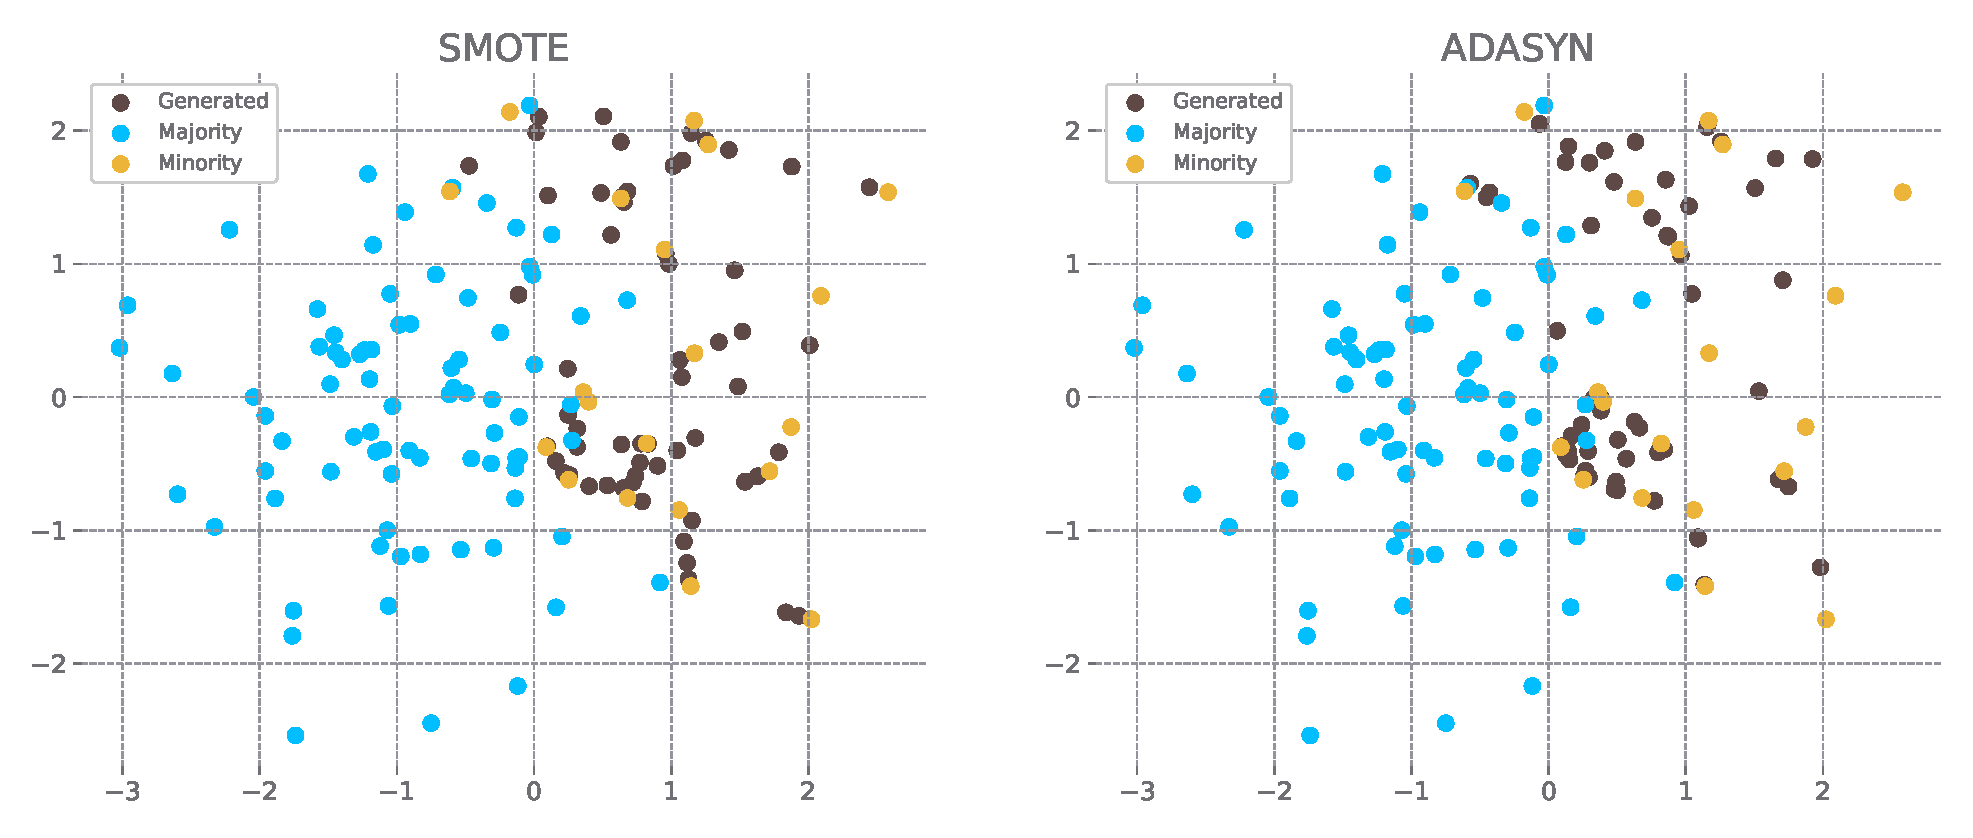
\includegraphics[width=\linewidth]{figures/smote_vs_adasyn.eps}
    \caption{
        \textbf{SMOTE vs ADASYN.} The figure shows how ADASYN, shown on the right, shifts new
        artificial samples towards the majority class as classification is more challenging in
        those regions. ADASYN generates almost no new samples on the right side of the plot,
        whereas SMOTE generates a few.
    }
    \label{figure:smote-vs-adasyn}
\end{figure}


\section{Undersampling Methods}
\label{section:undersampling-methods}

Undersampling methods focus on the majority class, as opposed to the oversampling methods discussed
in Section \ref{section:oversampling-methods}, to address the issue of the imbalanced
classification. These methods reduce the number of samples in the majority class to create a more
balanced distribution of samples between classes. Most of the undersampling methods discussed are
so-called \textit{prototype selection} methods. Prototype selection methods reduce the number of
samples by removing unnecessary samples from the dataset and using only a subset of the original
data. The Cluster Centroids method is the only example of a \textit{prototype generation} method
discussed in the thesis. Prototype generation methods reduce the number of samples by generating
new samples, e.g. centroids of clusters obtained by the KMeans algorithm~\ref{section:kmeans},
instead of using a subset of the original ones.


\subsection{Random Undersampling}
\label{subsection:random-undersampling}

Random undersampling works on the samples from the majority class. It works similarly to the Random
oversampling discussed in~\ref{subsection:random-oversampling}, but instead of duplicating the
randomly chosen samples, it removes them until the required number of samples is achieved.


\subsection{Condensed Nearest Neighbour}
\label{subsection:cnn}

Condensed Nearest Neighbour rule~\cite{cnn} has been proposed to reduce the nearest neighbour
rule's stringent storage requirements, retaining the basic idea of the nearest neighbour rule. The
nearest neighbour rule works with the so-called stored reference set consisting of n examples that
are correctly classified beforehand, for example, by a human annotator. A new sample is assigned
the same class as its nearest neighbour in the reference set. The CNN rule reduces this potentially
huge reference set to a \textit{consistent} set. The consistent set is a subset of the original
reference set. When used as the reference set in the NN rule, it correctly classifies all of the
examples from the original reference set. CNN rule uses two sets called \texttt{STORE} and
\texttt{GRABBAG} and works as follows:

\begin{enumerate}
    \item initialise \texttt{STORE} = \texttt{GRABBAG} = \{\}
    \item store the first example in the \texttt{STORE} set
    \item classify the following example using only examples in the \texttt{STORE} set; if
        classified correctly, put it in \texttt{\texttt{GRABBAG}} otherwise, put it in
        \texttt{STORE}
    \item continue inductively, i.e. the ith example is classified using the contents of
        \texttt{STORE} and placed in \texttt{STORE} if misclassified, or in \texttt{GRABBAG} if
        classified correctly
    \item loop through the whole original reference set and continue looping through
        \texttt{GRABBAG} once the original set was processed wholly
    \item terminate when either the \texttt{STORE} equals the original reference set or when the
        \texttt{STORE} has not changed for one whole pass
    \item keep the \texttt{STORE} set and discard the \texttt{GRABBAG} set
\end{enumerate}

The CNN undersampling algorithm makes one change to this algorithm. It starts with \texttt{STORE} =
$S_{min}$ and loops through examples in the majority class.

\begin{figure}
    \centering
    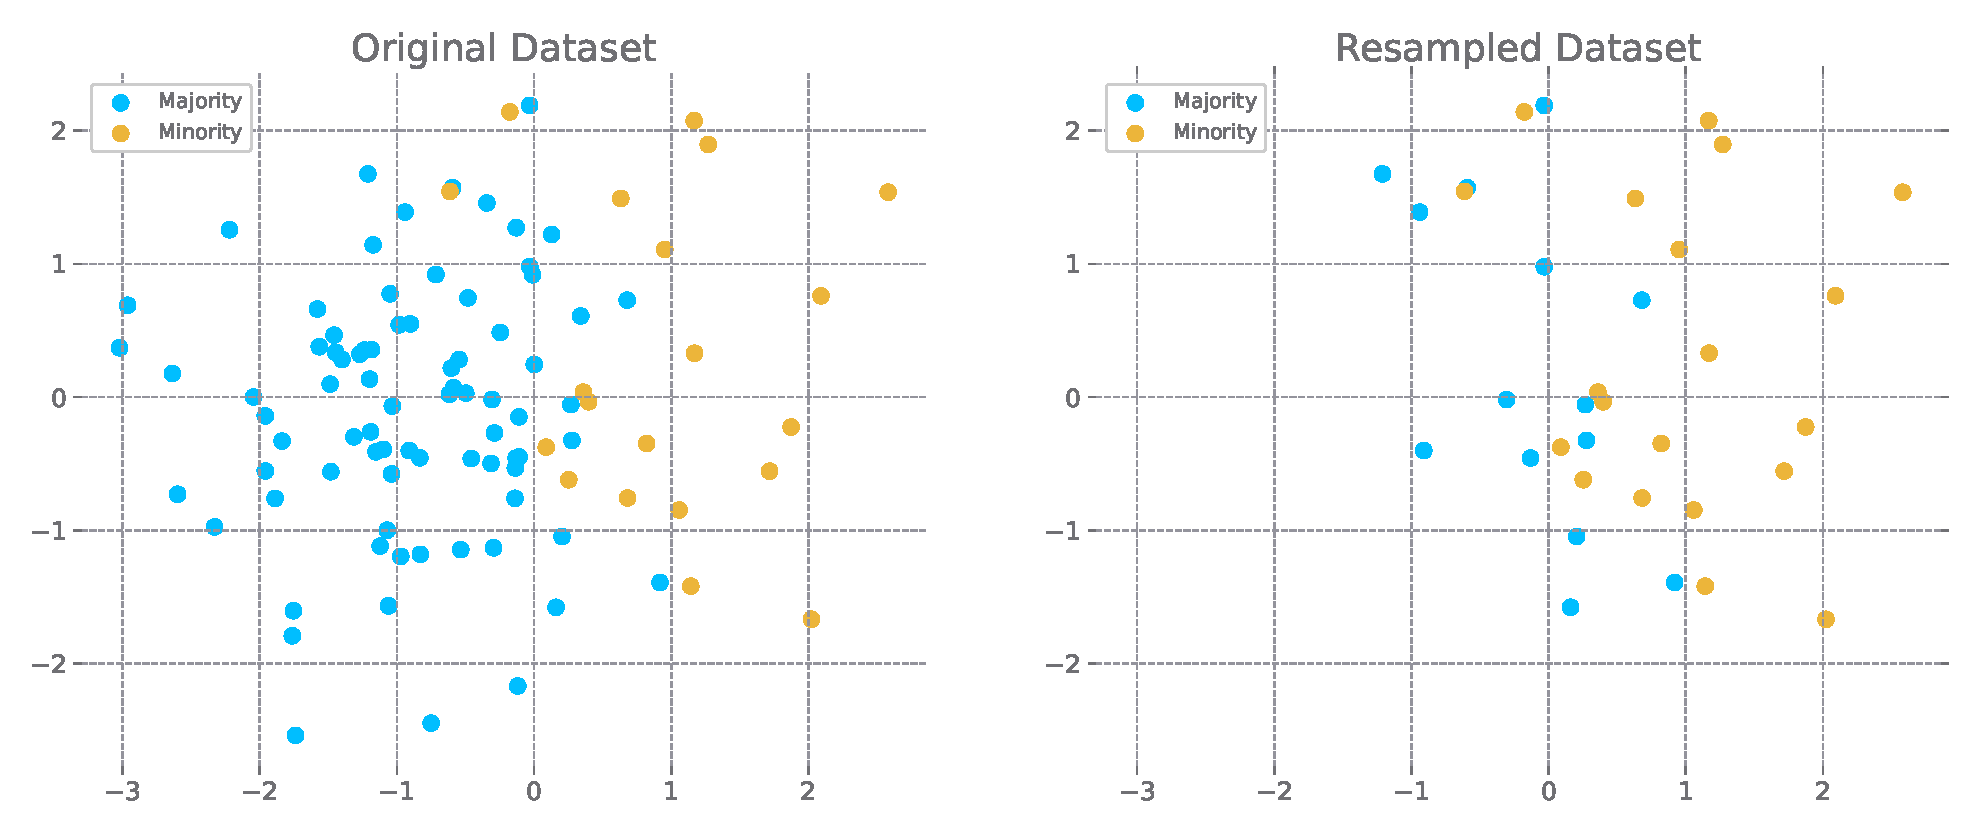
\includegraphics[width=\linewidth]{figures/cnn.eps}
    \caption{
        \textbf{Undersampling using Condensed Nearest Neighbour.} The figure shows the original
        data distribution on the left, the same data distribution after identifying samples to
        remove shown in brown colour and the resulting undersampled dataset on the right after
        applying the CNN method. With little overlap in the data, the CNN method discarded most
        samples from the majority class. It kept only samples close to the decision boundary needed
        to classify the remaining points correctly.
    }
    \label{figure:cnn}
\end{figure}


\subsection{Edited Nearest Neighbours \& Repeated ENN}
\label{subsection:enn}

We will now describe two other related modifications to the nearest neighbours algorithm. In the
first step, the Edited Nearest Neighbours algorithm~\cite{enn} proposed by Dennis L. Wilson
classifies all samples in the class to undersample by computing k-nearest neighbours for each on
the whole original set. The second step proceeds to remove all such samples under consideration
whose actual label does not match the label of most of their neighbours. We can see a plot showing
the ENN method in Figure~\ref{figure:enn}. Ivan Tomek proposed to repeat ENN multiple times to
reduce the number of majority samples further~\cite{repeated-enn}. The algorithm iteratively
reduces the number of samples in the majority class until there is no reduction in the number of
majority samples or the maximum number of iterations is reached. We refrain from showing a plot for
the Repeated ENN method, as in this particular case, ENN and Repeated ENN produced the same
results.

\begin{figure}
    \centering
    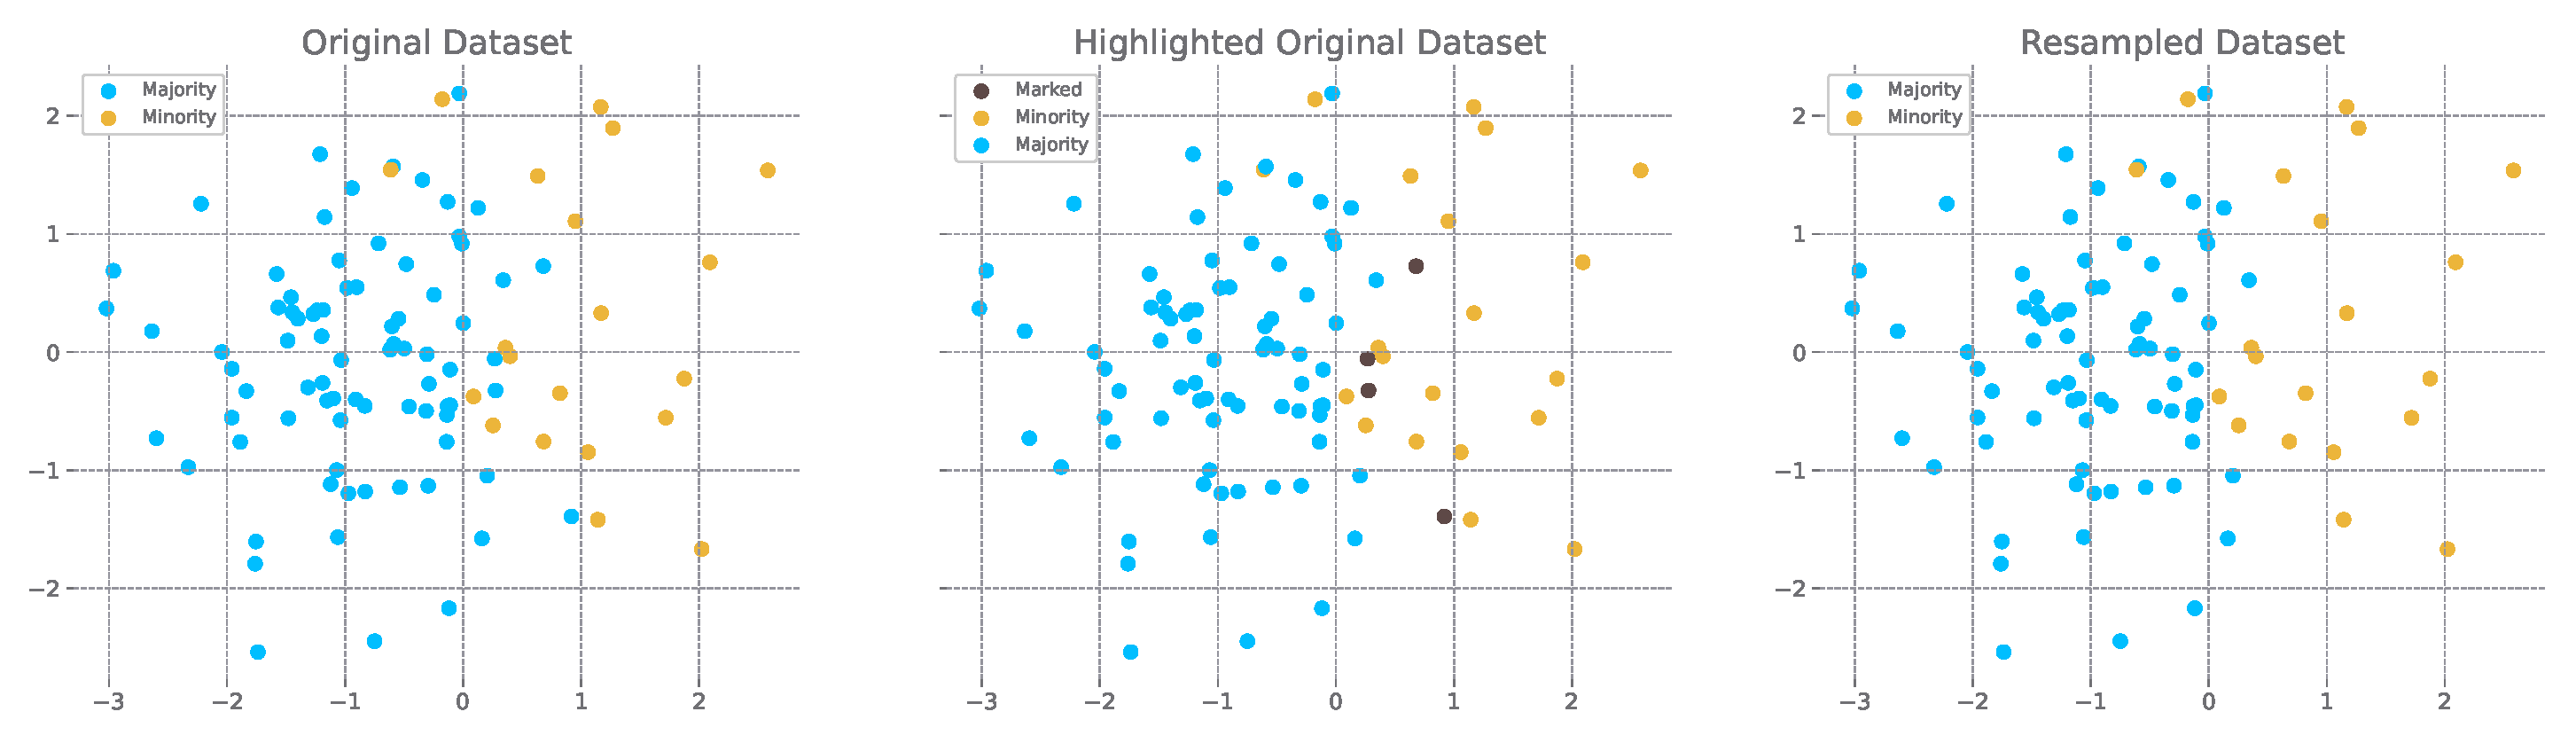
\includegraphics[width=\linewidth]{figures/enn.eps}
    \caption{
        \textbf{Undersampling using Edited Nearest Neighbours.} The leftmost plot shows the
        original dataset, and the rightmost plot shows the new undersampled one. The middle one
        shows data samples marked for removal in brown colour as computed by the ENN method with
        hyperparameter $k = 3$.
    }
    \label{figure:enn}
\end{figure}


\subsection{All KNN}
\label{subsection:allknn}

All KNN~\cite{repeated-enn}, also proposed by Ivan Tomek, uses the same idea as the two previous
preprocessing methods to eliminate samples from the majority class when there is a label
disagreement between a sample under consideration and its k-nearest neighbours. However, instead of
using a fixed number of neighbours to check an agreement, it starts by looking at the single
nearest neighbour, then two nearest neighbours and so on, until it reaches k-nearest neighbours. A
sample is kept in the majority class only if its label agrees in all cases. This idea can be
summarised in pseudocode in the following way:

\begin{algorithm}
    \caption{
        \textbf{A pseudocode representation of the All KNN algorithm.} The algorithm uses the
        \texttt{discard} set to store samples whose labels are inconsistent with the labels of
        their neighbours. It loops over all samples from the majority class and uses
        \textrm{NN}(\texttt{i}, \texttt{x}) to compute the \texttt{i}-nearest neighbours of sample
        \texttt{x}. Samples whose label is inconsistent with labels of \texttt{i}-nearest
        neighbours at any point are added to the \texttt{discard} set and removed from the
        \texttt{maj\_samples} set at the end of the algorithm.
    }
    \label{algorithm:all-knn}

    \begin{algorithmic}
        \Function{AllKNN}{$\texttt{maj\_samples}, \texttt{k}$}
            \State $\texttt{discard} \gets \{\}$

            \For{$\texttt{x}$ \textbf{from} $\texttt{maj\_samples}$}
                \For{$\texttt{i} \gets 1$ \textbf{to} $\texttt{k}$}
                    \State $\texttt{neighbours} \gets \textrm{NN}(\texttt{i}, \texttt{x})$

                    \If{$\texttt{x}$ is incorrectly classified using $\texttt{neighbours}$}
                        \State $\texttt{discard}.\textrm{add}(\texttt{x})$
                        \State \textbf{break}
                    \EndIf
                \EndFor
            \EndFor

            \State \Return $\texttt{maj\_samples} - \texttt{discard}$
        \EndFunction
    \end{algorithmic}
\end{algorithm}

\begin{figure}
    \centering
    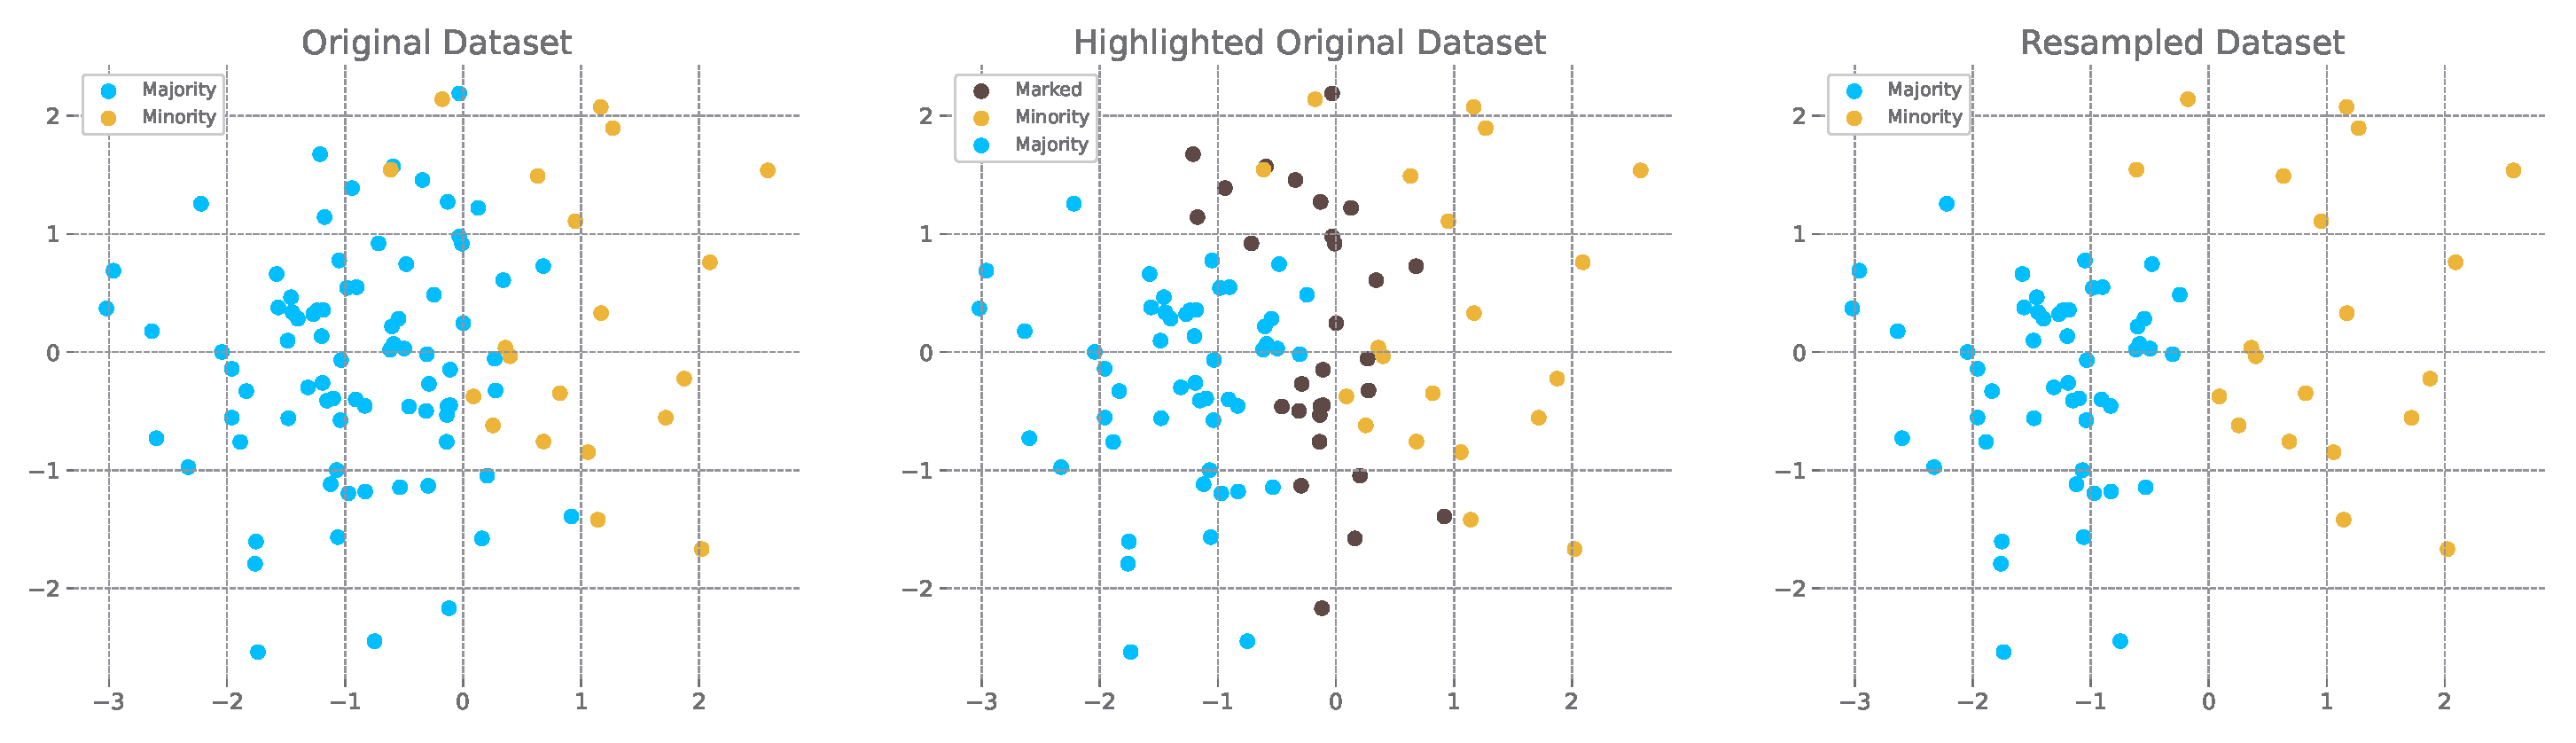
\includegraphics[width=\linewidth]{figures/all_knn.eps}
    \caption{
        \textbf{Undersampling using All KNN.} The figure shows the original dataset in the leftmost
        plot. The majority samples selected by the All KNN method with the hyperparameter $k = 7$
        are highlighted in the centre plot. The last plot shows the dataset after removing the
        highlighted samples from the middle plot. Note that for the purposes of illustration, we
        only kept the majority samples if their labels matched the labels of all their neighbours,
        as opposed to the described original approach.
    }
    \label{figure:all-knn}
\end{figure}


\subsection{Near Miss}
\label{subsection:near-miss}

Near Miss~\cite{near-miss} refers to a group of three undersampling methods that use kNN to select
majority class samples to retain. The three methods are Near Miss 1, Near Miss 2 and Near Miss 3.

\begin{enumerate}
    \item \textbf{Near Miss 1} selects majority samples that exhibit the smallest average distance
        to $\mathrm{N}$ closest minority samples
    \item \textbf{Near Miss 2} selects majority samples that exhibit the smallest average distance
        to $\mathrm{N}$ furthest minority samples
    \item \textbf{Near Miss 3} selects a given number of closest majority samples for each minority
        sample
\end{enumerate}

\begin{figure}
    \centering
    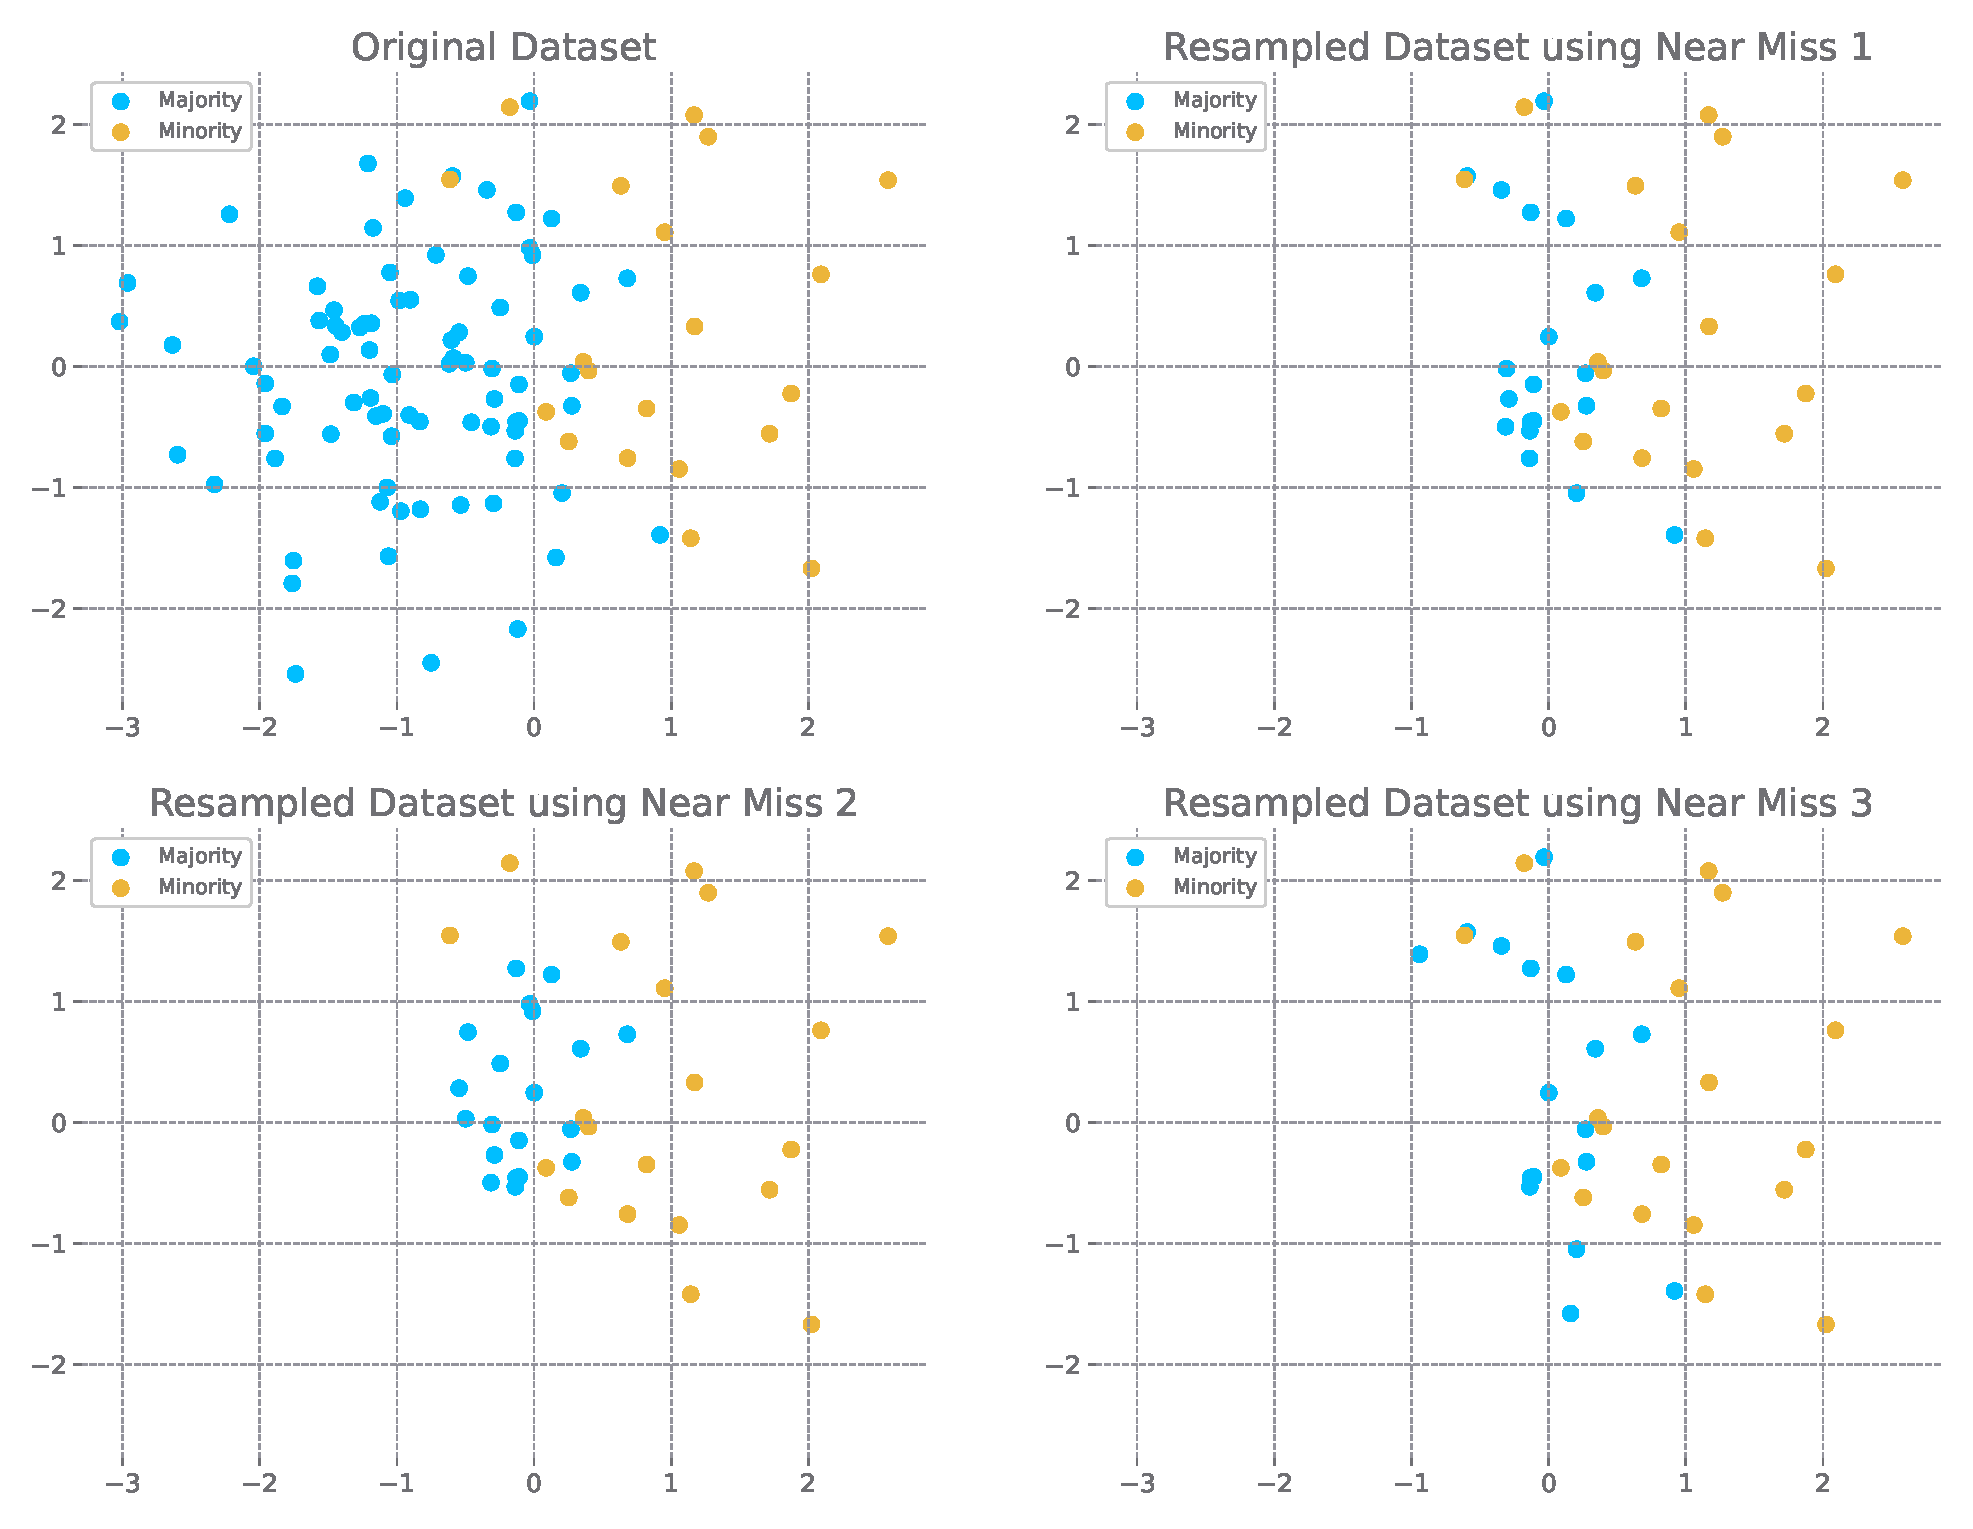
\includegraphics[width=\linewidth]{figures/near_miss.eps}
    \caption{
        \textbf{Undersampling using Near Miss 1, 2 and 3.} The plot shows the original dataset in
        the upper left corner and resulting dataset after applying each of the three Near Miss
        methods in the remaining plots.
    }
    \label{figure:near-miss}
\end{figure}


\subsection{Tomek Links}
\label{subsection:tomek-links}

Tomek Links~\cite{tomek-links} is a data cleaning technique used to clean the area near the
decision boundary and to remove noisy samples. A pair of points $\mathbf{x}_i~\in~S_{min}$,
$\mathbf{x}_j~\in~S_{maj}$ belonging to the opposite classes form a Tomek Link if there does not
exist a sample $\mathbf{x}_k$ such that $\mathrm{d}(\mathbf{x}_i, \mathbf{x}_k) \leq
\mathrm{d}(\mathbf{x}_i, \mathbf{x}_j)$ or $\mathrm{d}(\mathbf{x}_j, \mathbf{x}_k) \leq
\mathrm{d}(\mathbf{x}_i, \mathbf{x}_j)$. The algorithm identifies samples from the majority class
participating in the Tomek Links and removes them, achieving a more pronounced decision boundary
and cleaner data, as depicted in Figure~\ref{figure:tomek-links}. Tomek Links are often used after
an oversampling method, such as SMOTE~\ref{subsection:smote}, to remove noisy samples introduced
during oversampling~\cite{learning-from-imb-data, batista2004}.

\begin{figure}
    \centering
    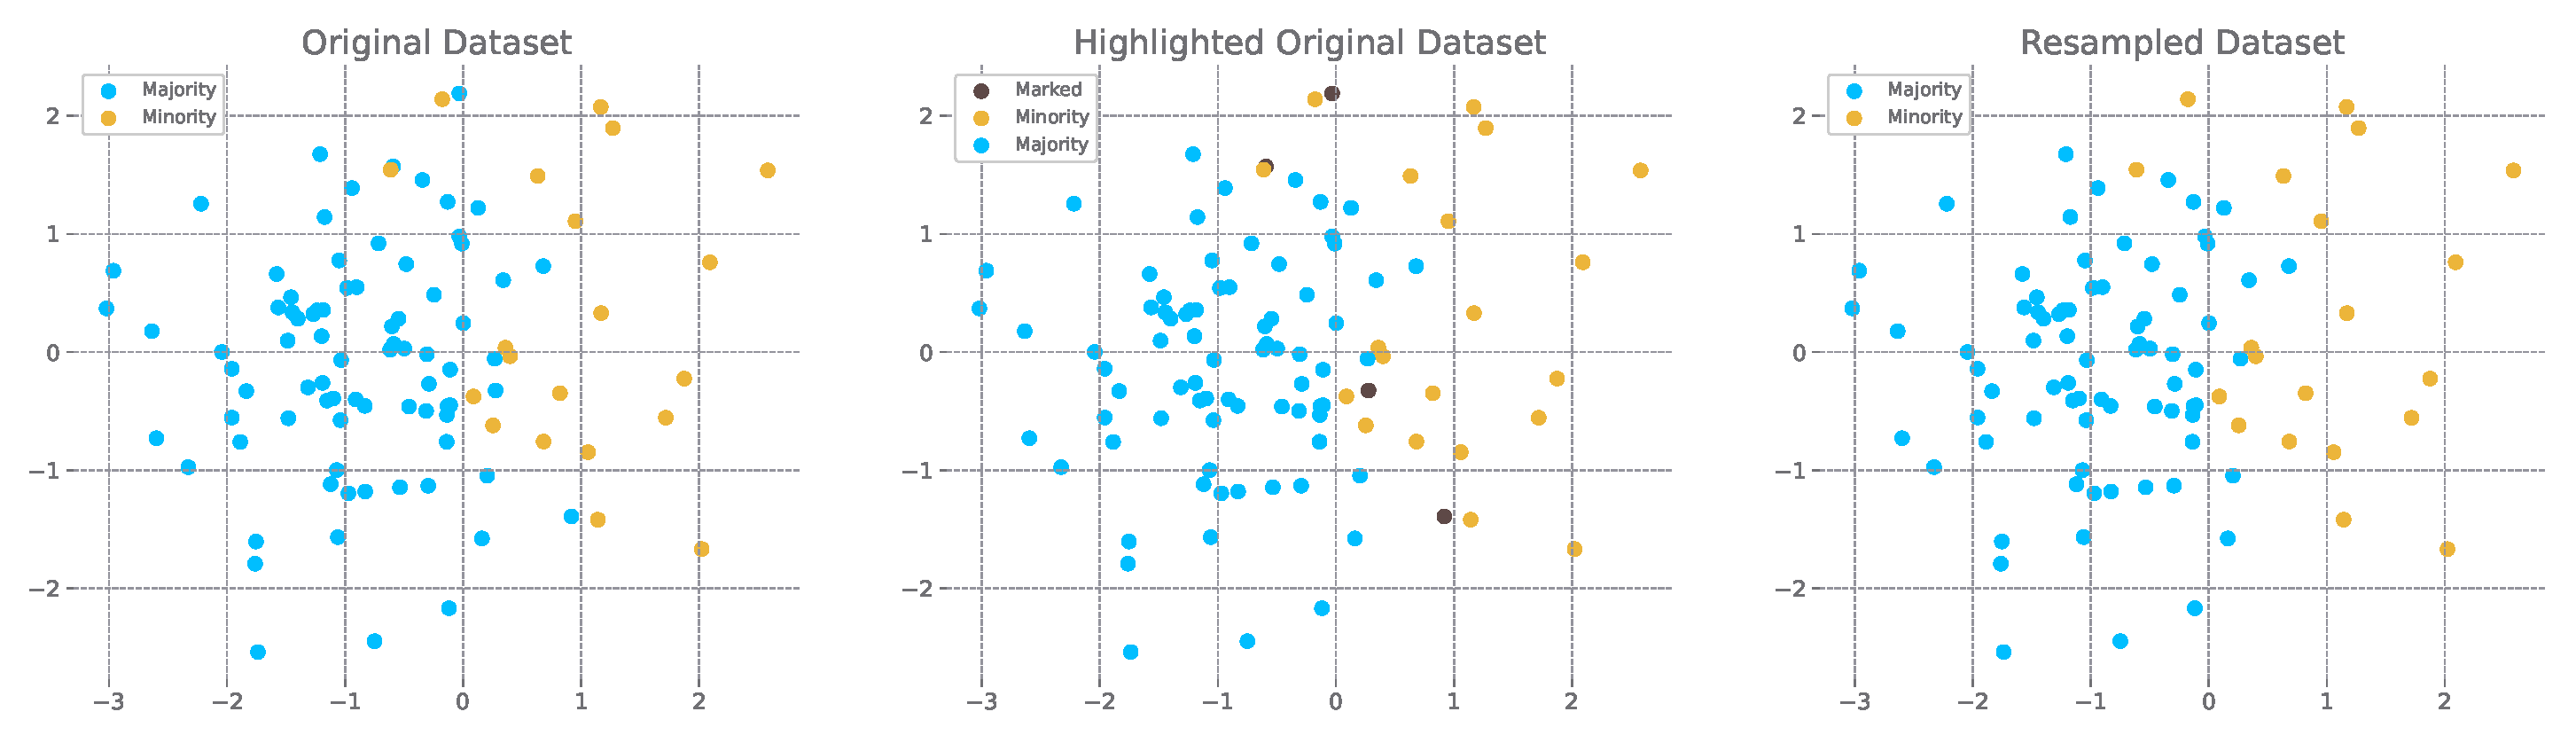
\includegraphics[width=\linewidth]{figures/tomek_links.eps}
    \caption{
        \textbf{Undersampling using Tomek Links.} The figure shows the Tomek Links cleaning method.
        The left plot shows the original dataset; the middle one reveals samples belonging to the
        majority class identified as Tomek Links in brown colour. Finally, the rightmost plot
        displays the cleaned dataset.
    }
    \label{figure:tomek-links}
\end{figure}


\subsection{One-Sided Selection}
\label{subsection:one-side-selection}

Authors of the One-Sided Selection algorithm~\cite{one-sided-selection} developed a clever
classification of majority samples into four categories. We describe these four categories below
and depict them in Figure~\ref{figure:oss}.

\begin{enumerate}
    \item \emph{Noise samples} - usually samples surrounded by the opposite class
    \item \emph{Borderline samples} - samples lying on the decision boundary
    \item \emph{Redundant samples} - samples lying far away from the decision boundary
    \item \emph{Safe samples} - rest of the samples that are worth keeping
\end{enumerate}

Moreover, the authors use the fact that noise and borderline samples can easily be recognised using
Tomek Links methods~\ref{subsection:tomek-links}, and redundant samples can be removed using the
idea discussed in Condensed Nearest Neighbours method~\ref{subsection:cnn}. The algorithm starts by
finding the consistent subset $C$ of the original set by performing a single iteration of the CNN
algorithm. Consequently, it identifies Tomek Links in $C$ and removes only the majority class
samples participating in the Tomek Links while retaining all minority samples.

\begin{figure}
    \centering
    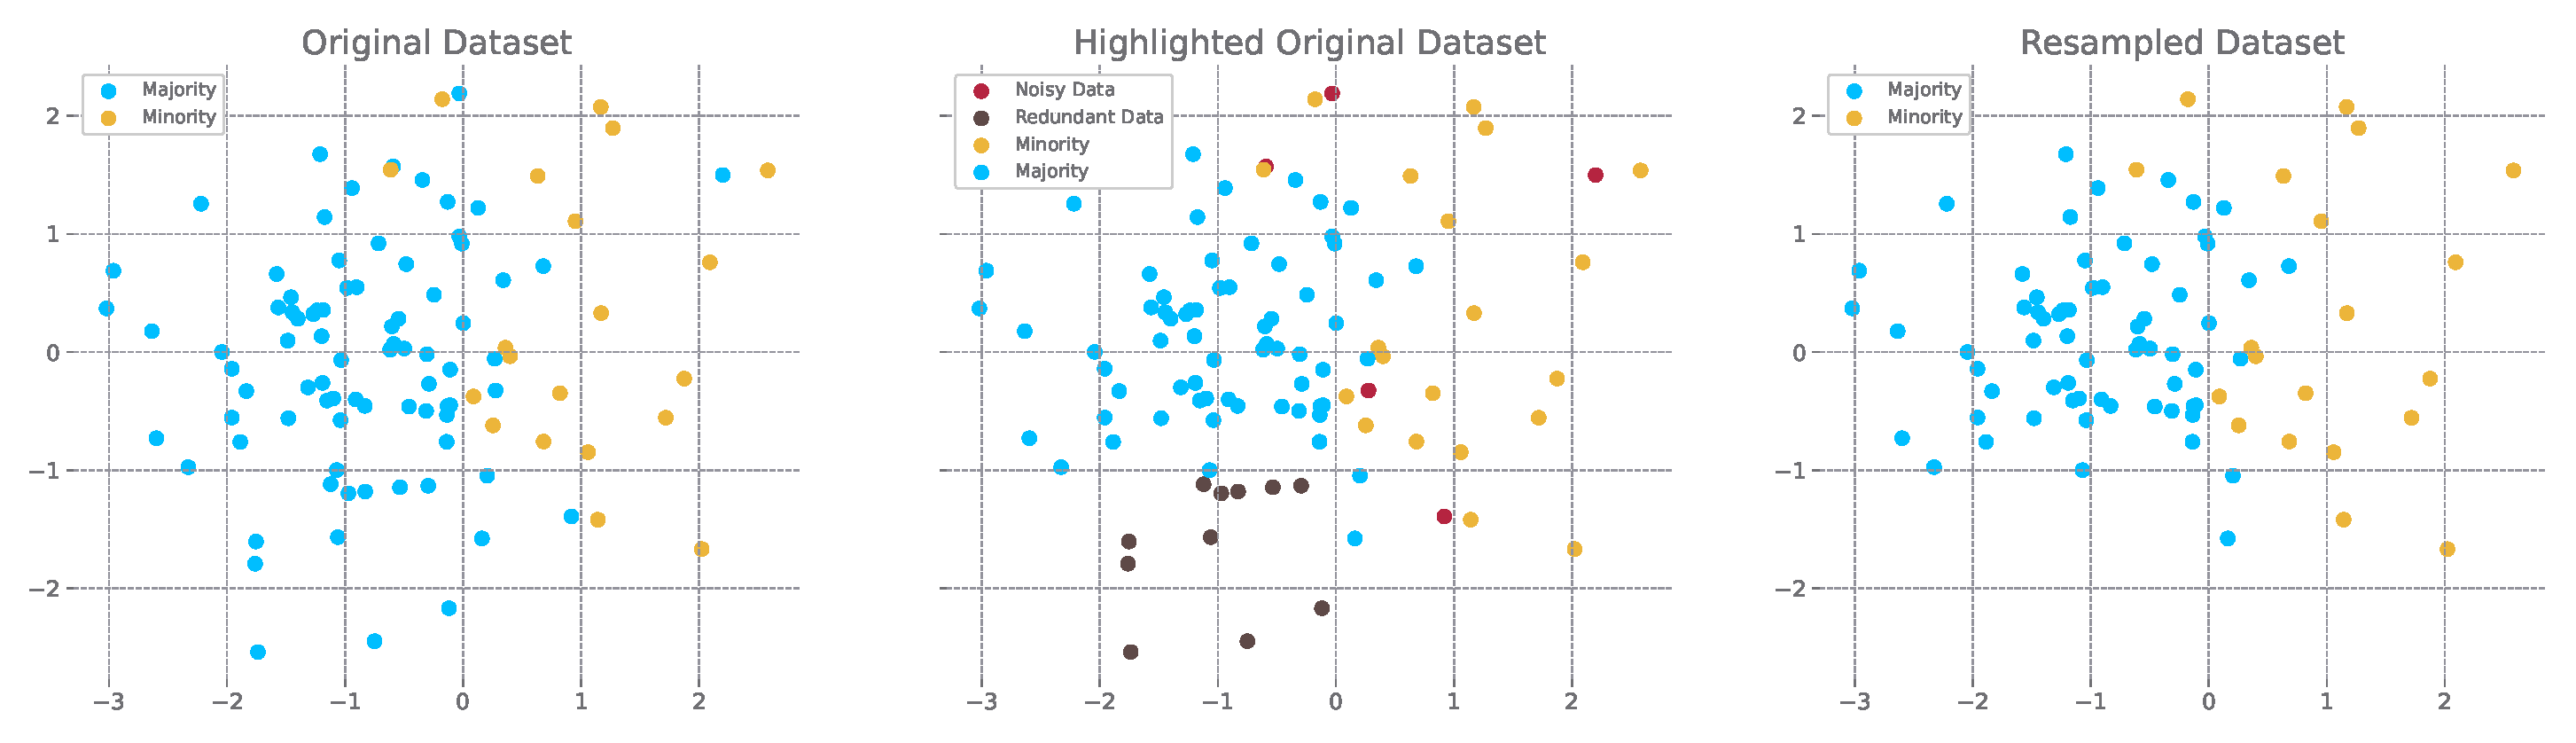
\includegraphics[width=\linewidth]{figures/oss.eps}
    \caption{
        \textbf{Undersampling using One-Sided Selection.} The figure shows the original data on the
        left. The scatter plot in the middle shows the borderline samples identified by the Tomek
        Links method highlighted in red and redundant samples identified using one iteration of CNN
        in brown. A single noisy sample is also identified using Tomek Links in the upper right
        corner. The rightmost scatter plot shows the resulting undersampled dataset.
    }
    \label{figure:oss}
\end{figure}


\subsection{Neighbourhood Cleaning Rule}
\label{subsection:neighbourhood-cleaning-rule}

Neighbourhood Cleaning Rule~\cite{ncl} tries to mitigate one major drawback of the One-Sided
Selection method discussed previously in Subsection~\ref{subsection:one-side-selection}. One-Sided
Selection uses the CNN method~\ref{subsection:cnn}, which is extremely sensitive to noise,
retaining noisy samples in the training set~\cite{ncl}. It uses the ENN method~\ref{subsection:enn}
instead of CNN to remove the first batch of noisy data. Additionally, NCL cleans the neighbourhoods
of minority samples. For each minority sample, it computes its three-nearest neighbours. If those
neighbours misclassify the minority sample under consideration, it removes the neighbours of that
sample that belong to the majority class.

\begin{figure}
    \centering
    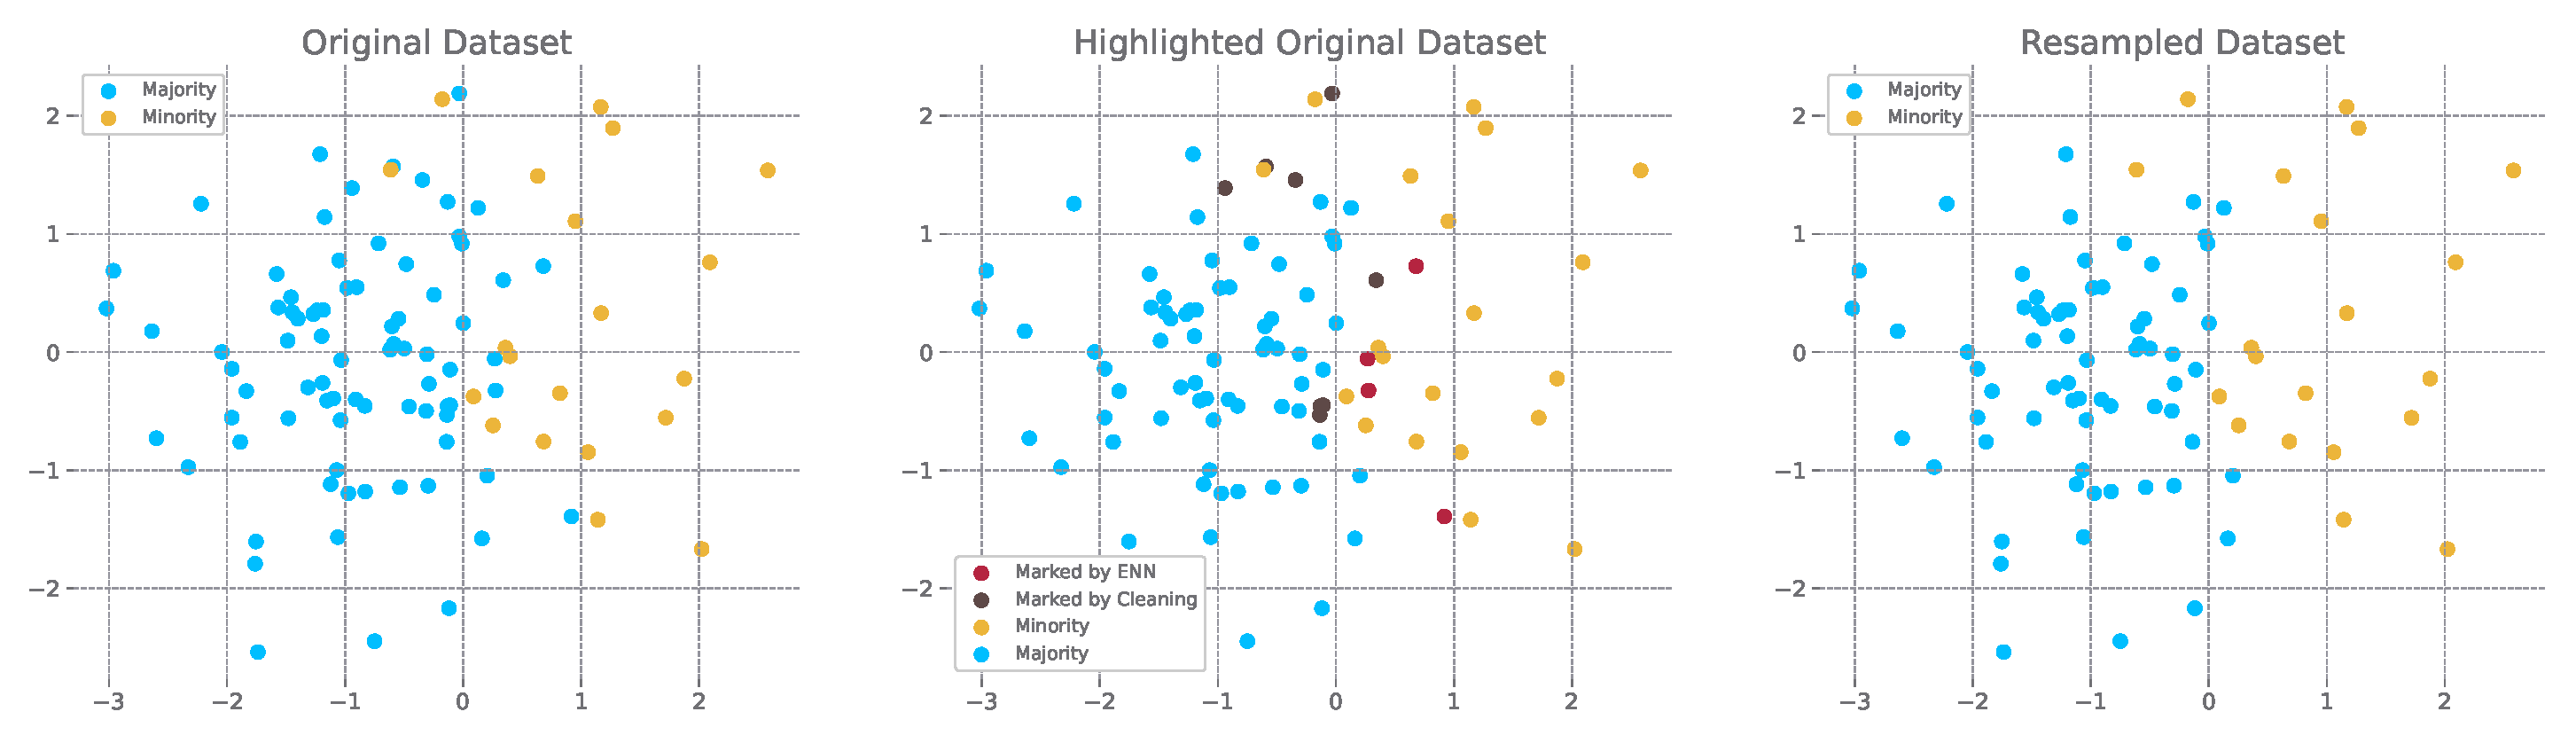
\includegraphics[width=\linewidth]{figures/ncl.eps}
    \caption{
        \textbf{Undersampling using Neighbourhood Cleaning Rule.} The figure depicts a process of
        undersampling using the Neighbourhood Cleaning Rule. It starts with the original dataset on
        the left, continues with the original dataset with data samples to remove marked in red and
        brown colours and finishes with the resampled dataset. In the middle plot, we can see that
        the data points identified as redundant by ENN are shown in red. The brown data points are
        to be removed in the subsequent step as they hinder the classification of minority samples
        using the three-nearest neighbour rule. It is best seen in the top portion of the plot
        where all three nearest neighbours of the minority sample located approximately at the
        point $(-0.5, 1.5)$ are shown in brown and missing in the following plot.
    }
    \label{figure:ncl}
\end{figure}


\subsection{Cluster Centroids}
\label{subsection:cluster-centroids}

Cluster Centroids~\cite{cluster-centroids} is a method belonging to the category of prototype
generation methods. Instead of selecting a subset of existing majority class samples, it
synthesises new samples from the existing ones. As its name suggests, the cluster centroids method
uses centres of clusters as the new undersampled data. It runs KMeans clustering
algorithm~\ref{section:kmeans} on the majority class with an appropriate number of clusters to
achieve the desired resulting ratio of samples belonging to individual classes. Once the KMeans
algorithm finishes, we output the cluster centroids as new majority class data.

\begin{figure}
    \centering
    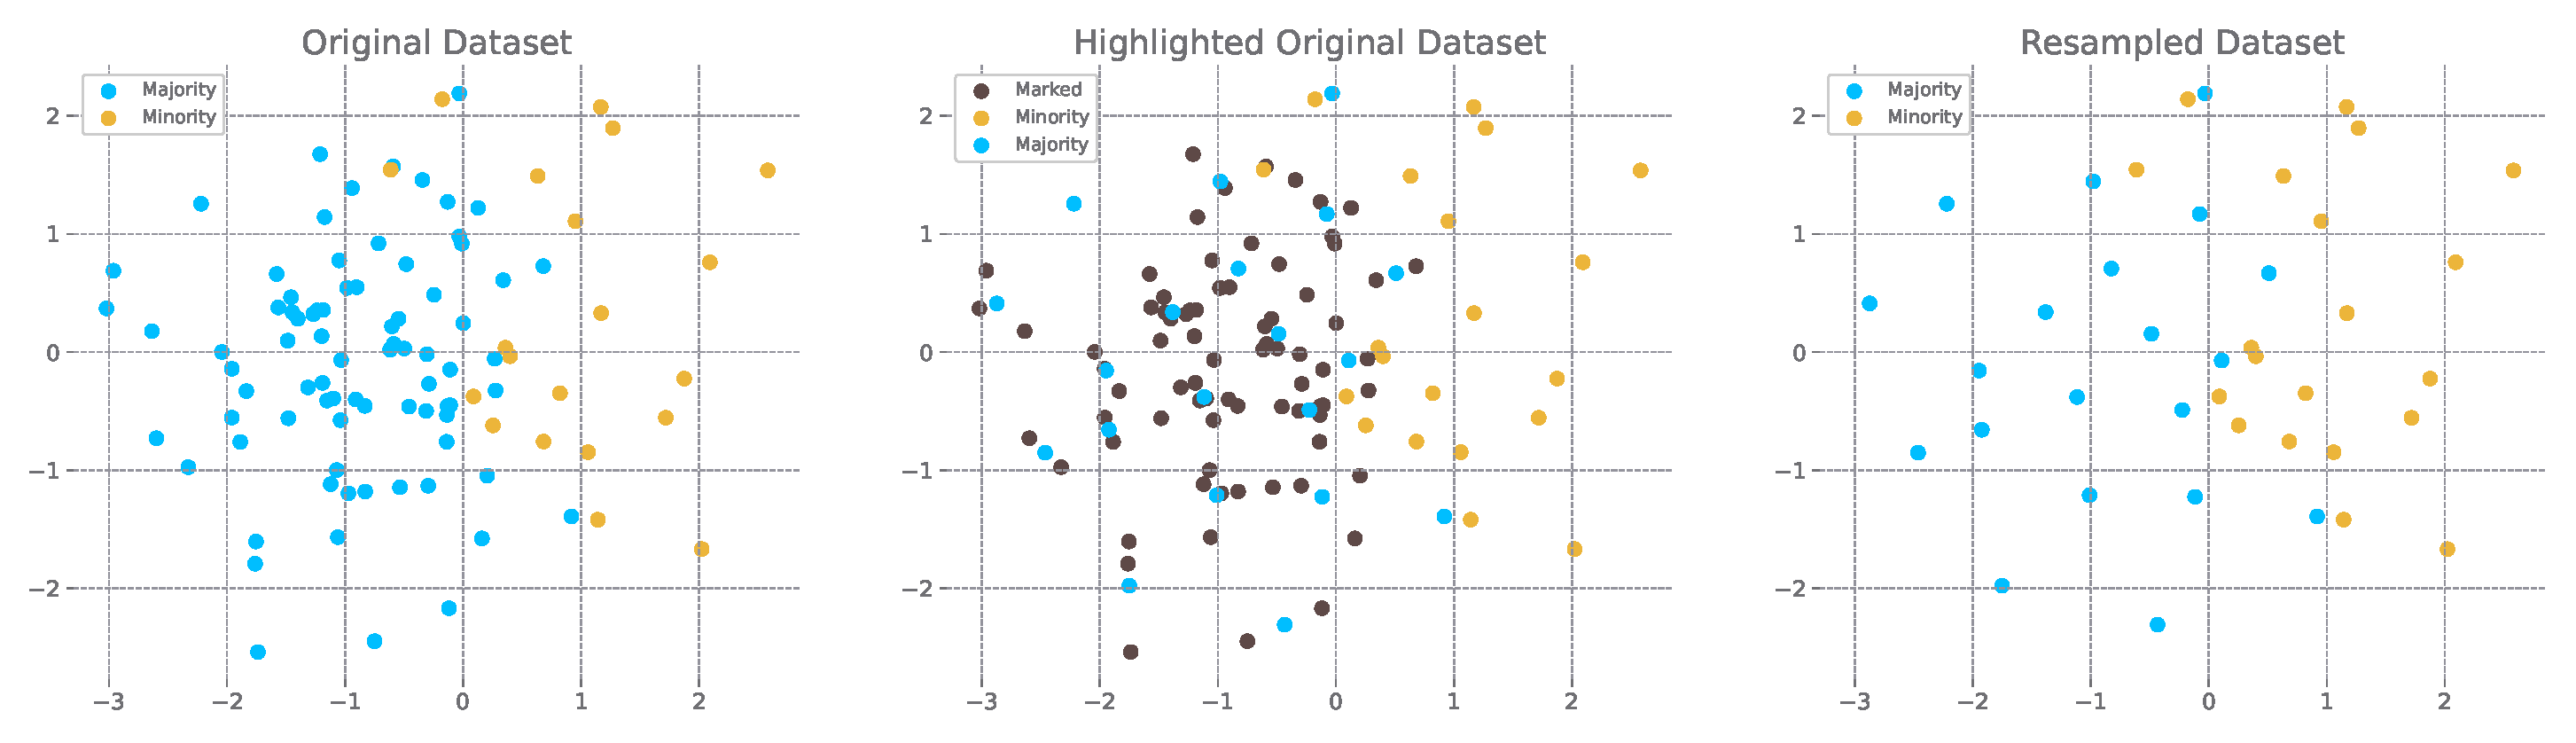
\includegraphics[width=\linewidth]{figures/cluster_centroids.eps}
    \caption{
        \textbf{Undersampling using Cluster Centroids.} The figure shows how the Cluster Centroids
        algorithm balances the distribution of samples between classes by creating new samples that
        are centroids of clusters found within the original majority class data and discarding the
        original majority class data. We can see how the new data points, shown in blue in the
        middle plot, are not present in the original dataset shown in the left plot. For example,
        there is a new majority example near the point $(-1.8, -2)$ in the central plot, whilst
        there is no such sample in the original dataset.
    }
    \label{figure:cluster-centroids}
\end{figure}
